\documentclass[a4paper]{jpconf}
%\bibliographystyle{iopart-num}
%\usepackage{citesort}
\usepackage{listings}
\usepackage{graphicx}

\lstset{ % General settings
language=c++,                   % choose the language of the code
basicstyle=\ttfamily \scriptsize,    % the size of the fonts that are used for the code \footnotsize
showspaces=false,               % show spaces adding particular underscores
showstringspaces=false,         % underline spaces within strings
showtabs=false,                 % show tabs within strings adding particular underscores
frame=,                         % adds a frame around the code (single)
tabsize=2,                      % sets default tabsize to 2 spaces
captionpos=t,                   % sets the caption-position: top (t), bottom (b)
breaklines=true,                % sets automatic line breaking
breakatwhitespace=false,        % sets if automatic breaks should only happen at whitespace
escapeinside={\%*}{*)},         % if you want to add a comment within your co>de
caption=footnote, 
label=listing:relRef
}

\begin{document}
\title{Ideal $\tau$ tagging with TMVA multivariate data-analysis toolkit}

\author{A Heikkinen, P Kaitaniemi, V Karim\"{a}ki,
M~J Kortelainen, T~Lamp\'{e}n, S Lehti, T Lind\'{e}n and L Wendland} 

\address{Helsinki Institute of Physics, P.O. Box 64, FIN-00014 University of Helsinki, Finland}

\ead{aatos.heikkinen@cern.ch}


\begin{abstract}
We report our experience on using ROOT package TMVA for
multivariate data analysis, for a problem of $\tau$ tagging in the
framework of heavy charged MSSM Higgs boson searches at the LHC.
With a generator level analysis,
we investigate how in the ideal case $\tau$ tagging could be performed and
hadronic $\tau$ decays separated from the
hadronic jets of QCD multi-jet background present in LHC experiments.
A successful separation of the Higgs signal from the background
requires a rejection factor of $10^5$ or better against the QCD background.
The $\tau$ tagging efficiency and background rejection are studied with various MVA classifiers.
\end{abstract}


\section{Introduction}


Our motivation stems from experience on using ROOT package TMVA for multivariate data analysis
\cite{chep07tmva}.
The chosen use case is $\tau$ tagging in the
framework of heavy charged MSSM Higgs boson searches at the LHC and our
goal is
to investigate how in the ideal case (no detector effects) $\tau$ tagging could be performed and 
signal $\tau$s separated from the background.


More substantial set of Monte Carlo data was prepared compared to our previous study.
This data consists a generator level Pythia/Tauola data for  14 TeV  p-p collisions:
signal is hadronic $\tau$ decay and
background consists of hadronic jets from QCD multi-jets (p$\mathrm{_T}$ = 120-170 GeV/c).


%Method/Results
The $\tau$ tagging efficiency and 
background rejection are studied with various MVA classifiers.
Moderate customisation was required to map our problem into the TMVA framework.

\section{TMVA - Toolkit for Parallel Multivariate Data Analysis}

ROOT-integrated TMVA is a framework the training, testing and performance evaluation
of multivariate classification techniques.
TMVA works in transparent factory mode 
to guarantee an unbiased performance comparison between the classifiers, such as:

\begin{itemize}
\item Rectangular cut optimisation
\item Projective likelihood estimation (PDE approach)
\item Multidimensional probability density estimation (PDE - range-search approach)
\item Multidimensional k-nearest neighbour classifier

\item Function discriminant analysis (FDA)
\item Predictive learning via rule ensembles (RuleFit)
\end{itemize}
 

\vspace{0.5cm}
In this presentation, we are focusing to following classifiers:
\begin{itemize}
\item Linear discriminant analysis (LDA) based on H-Matrix and Fisher discriminants
\item Boosted/Bagged decision trees (BDT)
\item Support Vector Machine (SVM) 
\item Artificial neural networks (ANN)
\end{itemize}


\section{Data}

The data for  dominating QCD multi-jet background was generated using Pythia8.108 for LHC 14 TeV p-p collisions.
The signal  was generated with Pythia6.4.19,
and required to consist only of genuine $\tau$ jets from the 
(heavy charged) MSSM $H^{\pm} \rightarrow \tau^{\pm}\nu_{\tau}$ decay 
with $\tau$ polarization simulated with Tauola 2.6~\cite{taola}.
In our maximal $m_H$ SUSY 
scenario \cite{maxsusy}  $m_{H_{\pm}}=217~GeV/c^2$ and $\tan\beta = 30$.

Our analysis is based on the variables listed in Table~\ref{tab:variables}.

%\begin{center}
%\begin{table}[h]
%\caption{\label{opt}Summary of {\sf QGSP\_\-INCL\_ABLA} physics list.}
%\footnotesize\rm
%\centering
%\begin{tabular}{@{}*{7}{l}}
%\br
%Option&Description\\
%\mr
%\verb"Al-"&Targets heavier than Aluminium.\\
%\verb"150~MeV -"&Projectile energies from $\sim$ 150 MeV up to 2.5 GeV $\sim$ 3 GeV.\\
%\br
%\end{tabular}
%\label{tab:AH:::}
%\end{table}
%\end{center}



\begin{table}[h]
\begin{center}
\caption{\label{tab:variables}Variables used in the analysis.}
\begin{tabular}{l*{2}{l}r}
%\hline
\br
Variable                                                  & Name                   \\
%\hline
\mr
Jet $E_T$                                                 & {\tt jetEt}            \\
Jet $\eta$                                                & {\tt jeteta}           \\
Track isolation ($\Delta$R=0.50)                          & {\tt isolMaxPt50}      \\
Isolation of electromagnetic energy ($\Delta$R=0.10 - 0.50) & {\tt ecalIsolEt10\_50} \\   
Neutral hadron rejection                                  & {\tt hcalRatio}        \\
(i.e. track p matching to hadronic energy deposition)     &                        \\
$R_{\tau}$ = p(leading track) / E(jet)                    & {\tt rtau}             \\
%\hline
\br
\end{tabular}
\end{center}
\end{table}



\subsection{Production and Preselection Cuts}

At Monte Carlo level the following preselection cuts were 
used following guidelines previously published for $\tau$ jet tagging \cite{tautagging} and 
$H^{+} \rightarrow \tau  \nu$~\cite{htau}:
\begin{itemize}
\item {\tt jetEt $>$ 100} (Fig.~\ref{fig:variables})
\item {\tt abs(jeteta) $<$ 2.2} 
\item Jet leading track p$_T$ $>$ 20 GeV, matching cone 0.1
\item Isolation:

\begin{itemize} 
\item track p$_T$ $>$ 0.5
\item {\tt abs(track $\eta$) $<$ 2.5}
\item {\tt abs(d$_{IP}$-z) $<$ 0.2}
\item around the leading track:
\begin{itemize}
\item signal cone $\Delta$R $<$ 0.04 
\item isolation cone 0.04 - 0.5 
\end{itemize} 
\item signal tracks 0, 1 or 2
\item isolation tracks 0 or 1
\end{itemize} 
\end{itemize} 

Further, before analysis we choose:
\begin{itemize}
\item 1-prong signal final states ({\tt signalTracks==1} )
\item MC matched $\tau$ jets coming from $H^{\pm}$ ({\tt tauDecayType==4})
\end{itemize}

\begin{figure}[h]
 \begin{minipage}{7.5cm}
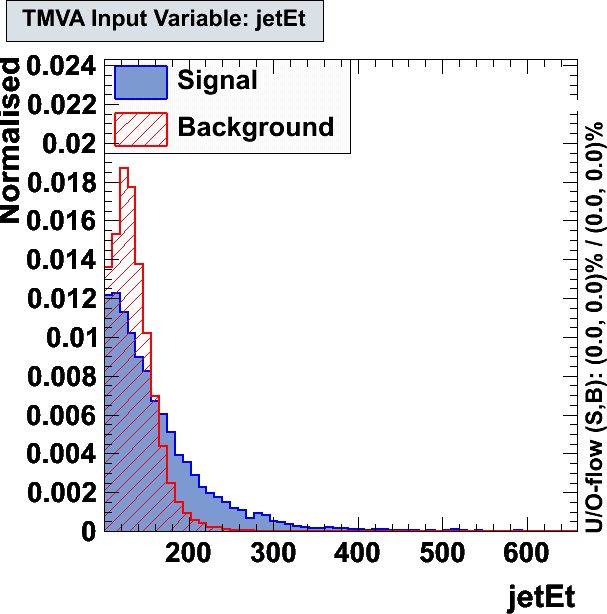
\includegraphics[width=0.9\textwidth]{images/jetet.png}
\end{minipage}
 \hfill
\begin{minipage}{7.5cm}
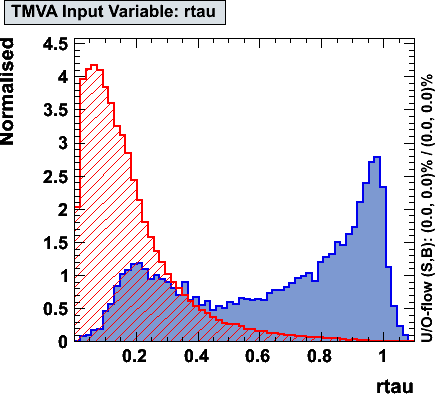
\includegraphics[width=1.0\textwidth]{images/rtau.png}
\end{minipage}
%\begin{minipage}{3.0cm}

\caption{Example of data used in $\tau$ tagging.
Distributions of jet $E_T$ ({\tt jetEt}) and $R_{\tau}$ ({\tt rtau}) variables are shown.}
%\end{minipage}
\label{fig:variables}
\end{figure}

%{\sf QGSP\_\-INCL\_ABLA} with

 
%\begin{figure}[h]
% \begin{minipage}{7.0cm}
%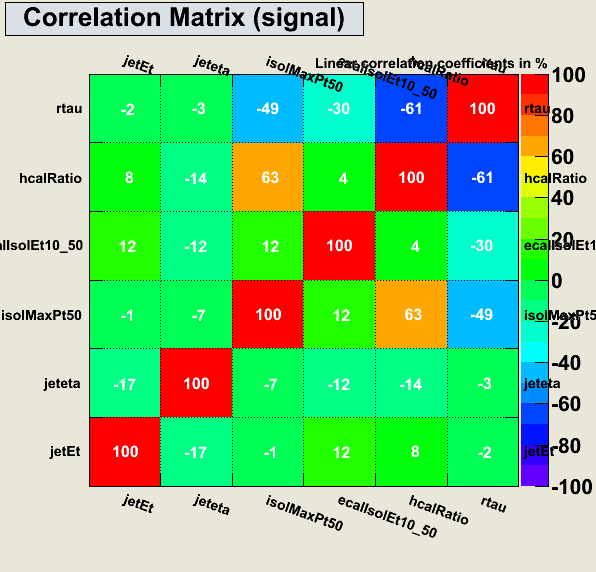
\includegraphics[width=1.0\textwidth]{images/ahCorrelationMatrixS.png}
%\end{minipage}
% \hfill
%\begin{minipage}{7.0cm}
%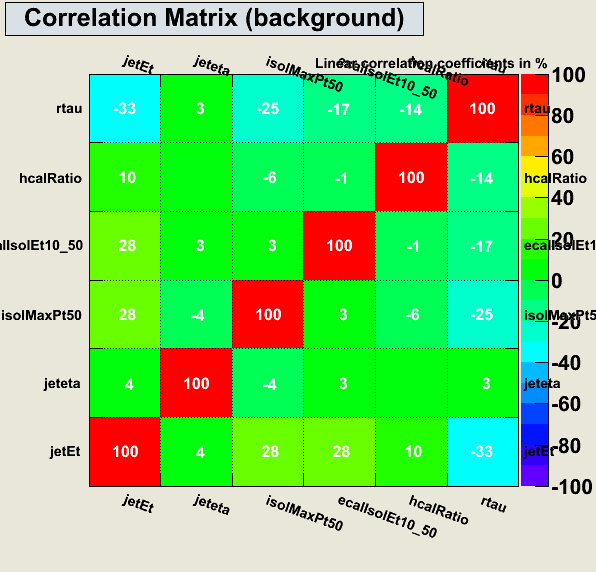
\includegraphics[width=1.0\textwidth]{images/ahCorrelationMatrixB.png}
%\end{minipage}
%\begin{minipage}{3.0cm}
%\caption{Right: Variable correlation matrix for signal Right: Variable correlation matrix for background}
%\end{minipage}
%\label{fig:ahCorrelationMatrix}
%\end{figure}

\section{Customisation of TMVA for $\tau$ tagging}

Customisation of TMVA included preparation of
configuration files, timing profiling with {\tt TStopwatch}
and evaluation of event efficiencies with {\tt TMVA::Reader}, taking into account
   the MC-level preselection efficiencies, and TMVA preselection efficiencies
Pseudo-pseudocode for the event evaluation is shown in  Appendix A Listing~\ref{listing:eventcode}.

Using signal (event) efficiency at background (event) efficiency level $10^{-5}$ and $10^{-6}$
Also we tabulating data related to  signal and background jet efficiency at $10^{-5}$
Example Listing~\ref{listing:log} in Appendix A from analysis run demonstrates these customisations.


\section{Results}

\subsection{Classifying with H-Matrix and Fisher discriminants}
Linear discriminant analysis  based on H-Matrix and Fisher discriminants
was performed with basic TMVA settings:

%Perusasetus, ei VarTransformia
%\scriptsize
\begin{verbatim}
Fisher H:!V:!Normalise:CreateMVAPdfs:Fisher:NbinsMVAPdf=50:NsmoothMVAPdf=1
HMatrix H:!V:CreateMVAPdfs
\end{verbatim}
%\normalsize

The response of TMVA to Fisher classifier id shown in Fig.~\ref{fig:fishersvm} 
%and \ref{fig:hmatrix},
and signal efficiencies are shown in Table~\ref{table:eff} together with other discrimination methods tested.
 

\begin{table}[h]
\caption{\label{table:eff}Summary of performance of various TMVA discriminators for the ideal $\tau$ tagging problem.}
\begin{center}
%\begin{tabular}{l*{2}{l}r}
\begin{tabular}{l*{2}{l}{l}r}
\br
Discriminator & Signal efficiency (\%) & \\
              & for background efficiency & \\
              &  $10^{-5}$    & $10^{-6}$              \\
\mr
H-Matrix & 1.1$\pm$0.5 (stat.) $\pm$ 0.1 (syst.)  & NN $\pm$ NN $\pm$ NN    \\
Fisher   & 3.5$\pm$0.9  $\pm$ 0.0   & NN $\pm$ NN $\pm$ NN  \\
BDT      & 7.8$\pm$0.1  $\pm$ 0.1(?)& 3.9$\pm$0.1 $\pm$ 0.1(?)\\
SVM      & 5.6$\pm$0.1  $\pm$ 0.1   & 1.7$\pm$0.1 $\pm$ 0.1   \\
MLP      & 7.6$\pm$0.2  $\pm$ 0.3   & 2.3$\pm$0.1 $\pm$ 0.3   \\
\br
\end{tabular}
\end{center}
\end{table}


\begin{figure}[h]
 \begin{minipage}{7.5cm}
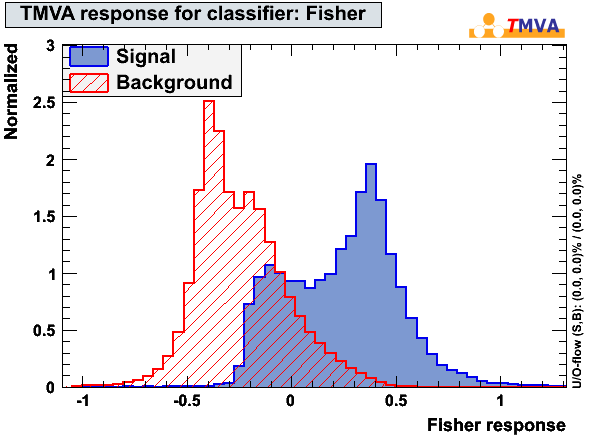
\includegraphics[width=1.0\textwidth]{images/mva_Fisher.png}
\end{minipage}
 \hfill
\begin{minipage}{7.5cm}
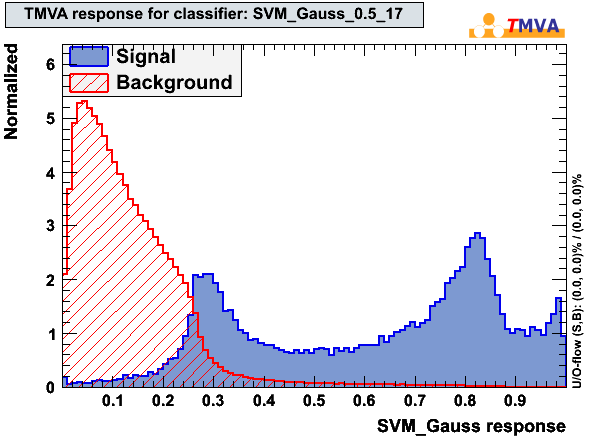
\includegraphics[width=1.0\textwidth]{images/mk_svm_gauss2.png}

%  \label{fig:mkSvmGauss2}
%\end{minipage}


\end{minipage}
%\begin{minipage}{3.0cm}
\caption{\label{fig:fishersvm}TMVA response to Fisher discriminant and 
the output of the SVM classifier with Gaussian kernel.}
%\end{minipage}
\end{figure}

%\begin{figure}[h]
%\begin{center}

%\caption{\label{fig:fisher}TMVA response to Fisher discriminant.}
%\caption{\label{fig:fisher}TMVA response to Fisher discriminant.}
%\end{center}
%\end{figure}

%\begin{figure}[h]
%\begin{center}
%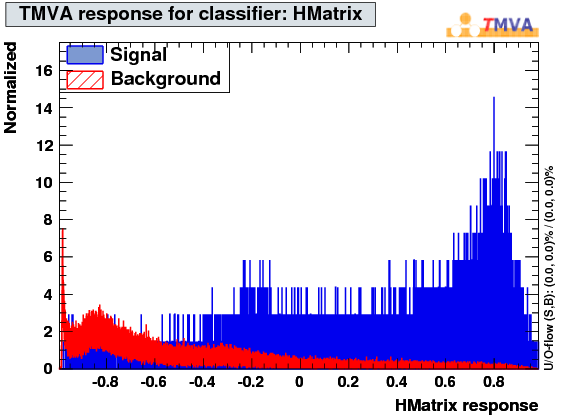
\includegraphics[width=0.8\textwidth]{images/mva_HMatrix.png}
%\caption{\label{fig:hmatrix}TMVA response to H-Matrix discriminant}
%\end{center}
%\end{figure}


\subsection{Boosted Decision Trees}

A decision tree is a binary tree classifier. 
Repeated left/right (yes/no) decisions are performed on a single variable at a time.
The phase space is split into regions that are classified as signal or
background, depending on the majority of training events that end up in the final leaf nodes.

Boosted Decision Trees (BDT) implemented in TMVA 
represents an extension to a single decision tree to several decision trees
derived from the same training sample by re-weighting events.
New combined classifier has stabilized response with respect to fluctuations in the training sample.

For our $\tau$ tagging problem the BDT method was found to give stable results 
with only small fluctuations (see Table~\ref{table:eff}).

\subsection{Support Vector Machine}
Support Vector Machine (SVM) in TMVA
was trained with 4k signal jets and 32k background jets.
The $\sigma, C$ parameter space
was optimized with 2D scan,  
a grid was set up in this space, and 
the training and evaluation for each point was run in parallel in a Linux cluster.

The SVM training time scales as O($n^2$), where $n$ is the number of events in the training sample  
and in practice training took $\sim$1 h. 
Figures 
%\ref{fig:mkSvmGauss2}
\ref{fig:fishersvm}
 and \ref{fig:mkSvmParallels} demonstrate the TMVA output of the SVM classifier
with Gaussian kernel.

%\begin{itemize}
%\item Training 4000 signal jets, 32000 background jets

%  \end{itemize}
%\item Results
%  \begin{itemize}
%  \item Background 1
%    \begin{itemize}
%    \item $10^{-5}$ bkg eff: $5.68\pm 0.12\;\%$
%    \item $10^{-6}$ bkg eff: $1.66\pm 0.06\;\%$
%    \end{itemize}
%  \item Background 2
%    \begin{itemize}
%    \item $10^{-5}$ bkg eff: $5.49\pm 0.12\;\%$
%    \item $10^{-6}$ bkg eff: $1.80\pm 0.07\;\%$
%    \end{itemize}
%
%  \end{itemize}
%\end{itemize}

 
%\begin{figure}[h]
% \begin{minipage}{7.0cm}
%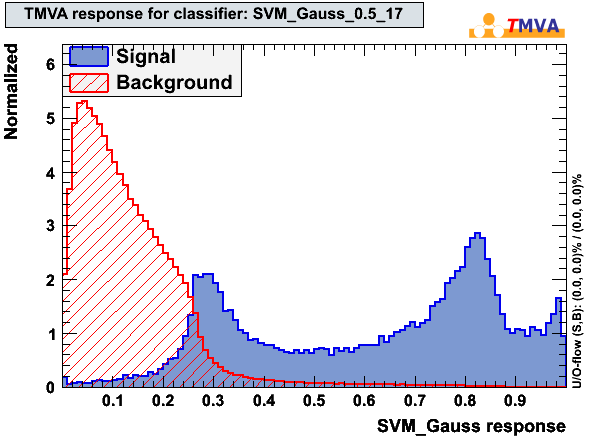
\includegraphics[width=0.8\textwidth]{images/mk_svm_gauss2.png}
%\end{minipage}
% \hfill
%\begin{minipage}{7.0cm}

%\end{minipage}
%\begin{minipage}{3.0cm}
%\caption{The output of the SVM classifier with Gaussian kernel.}
%  \label{fig:mkSvmGauss2}
%\end{minipage}

%\end{figure}


\begin{figure}[h]
\begin{center}
%\includegraphics[width=21pc]{poster/images/.png}\hspace{2pc}%
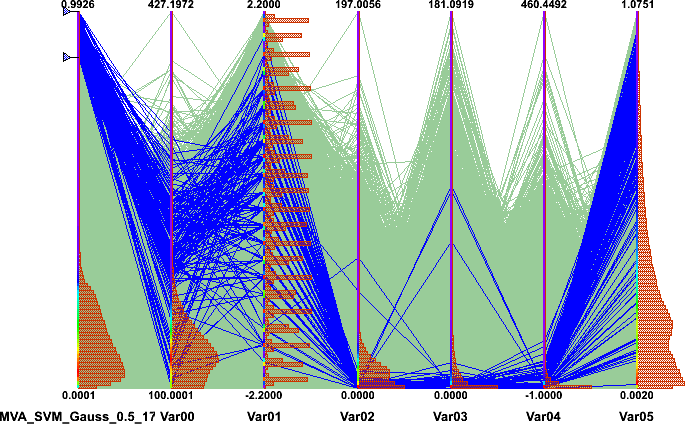
\includegraphics[width=1.0\textwidth]{images/svm_parallels2.png}
%\begin{minipage}[b]{14pc}
  \caption{TMVA plot for parallel coordinates. 
Poorly classified background events with value 0.9-1.0 are selected from vertical histogram on left. 
In this kind of plot each line going through variables represent on event, 
possibly giving insight to better variable selection.}
  \label{fig:mkSvmParallels}

%\end{minipage}
\end{center}
\end{figure}


\subsection{Neural Networks}

Of the three Multilayer Perceptrons (MLP) implementations supported by TMVA
we used ({\tt TMVA::Types::kMLP}).

Usual cariables {\tt jetEt, jeteta, isolMaxPt50, ecalIsolEt10\_50, hcalRatio}, and {\tt rtau}
were used. Results for MLP discriminator are shown for {\tt jetEt} transformation {\tt log(jetEt)} and 
Principal Component Analysis ({\tt  VarTransform=PCA}).

Data for 6-15-1 MLP configuration with neurons of sigmoid type we trained 1k cycles using
10k signal jets and 40k background jets. 
Rest of the data was used for testing (30k signal and 2230k background jets)
Systematic uncertainty was estimated by repeating the full analysis with independent background data.
Convergence of the neural network training and 
background rejection vs. signal efficiency plot  for test data are shown in Fig.~\ref{fig:nn}.

\begin{figure}[h]
 \begin{minipage}{7.5cm}
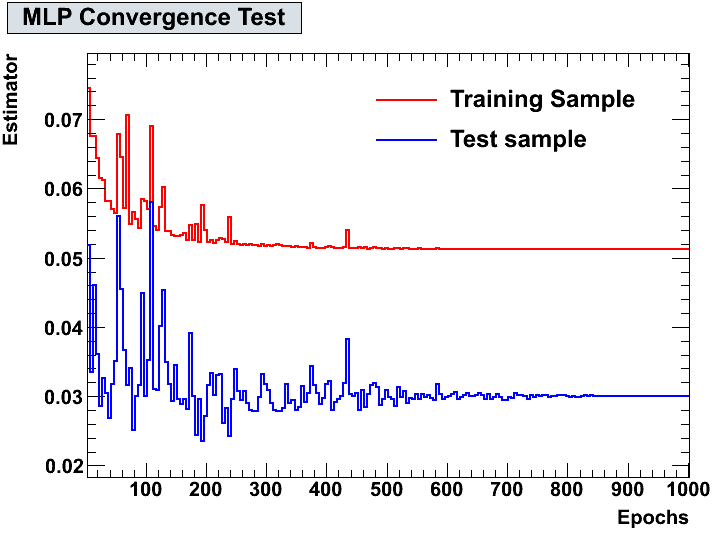
\includegraphics[width=1.0\textwidth]{images/MLPConvergenceTest.png}
\end{minipage}
 \hfill
\begin{minipage}{7.5cm}

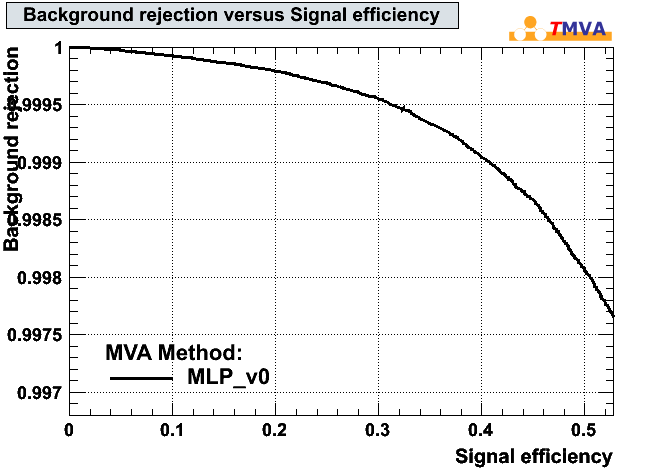
\includegraphics[width=1.0\textwidth]{images/roc.png}
\end{minipage}
%\begin{minipage}{3.0cm}
\caption{Convergence of ANN over 1000 training cycles and background rejection vs. signal efficiency.}
%\end{minipage}
\label{fig:nn}
\end{figure}

\section{Conclusion}
We have discussed from the user point of view how TMVA package in ROOT can be used in $\tau$ tagging.
We have seen that since CHEP'07 TMVA has matured, and is now fully integrated to ROOT
and an interface for adding new classifiers is provided.

Some customisation was needed to cast our problem into the TMVA framework.
We find multivariate data-analysis techniques show a promise in $\tau$ tagging.
At  $10^{-5}$ background efficiency, TMVA classifiers have 1.1-7.8~\% signal efficiency.
Finally, we have defined areas where our approach can be improved. 
(e.g. using additional variables, and yet unused classifiers available in TMVA), 
and are planning additional research on $\tau$ tagging


% \ack %command \ack sets the acknowledgments heading as an unnumbered section.


\appendix % The command \appendix" is used to signify the start of the appendixes.
\section{Customisation of TMVA event eavaluation}

\lstset{emph={Jog},emphstyle=\underbar,
caption=Pseudo-pseudocode for the event evaluation.,
breaklines=true,
stepnumber=99999,  %trick to remove line numbering
showlines=false,
label=listing:eventcode
}
\lstinputlisting{eventcode.txt}



\lstset{emph={Jog},emphstyle=\underbar,
caption=Example listing from TMVA analysis showing customisations done.,
breaklines=true,
stepnumber=99999,  %trick to remove line numbering
showlines=false,
label=listing:log
}
\lstinputlisting{log.txt}


%\begin{equation}
%time= money
%\end{equation}

%To obtain a simple heading of `Appendix' use the code \verb"\section*{Appendix}". 
%If it contains numbered equations, figures or tables the command \verb"\appendix" should
%precede it and \verb"\setcounter{section}{1}" must follow it. 


\section*{References}

\begin{thebibliography}{9}

%\bibitem{incl} A. Boudard et al., \emph{Intranuclear cascade model for
%    a comprehensive description of spallation reaction data}, Phys.
%  Rev. C66 (2002) 044615
%\bibitem{g4} \emph{Geant4 collaboration website} \\ {\tt http://\-cern.ch/\-geant4}
%\bibitem{pk08bProceedings}
%A. Heikkinen, P. Kaitaniemi, and A. Boudard,
%{\em Implementation of INCL4 cascade and ABLA evaporation codes in Geant4},
%Journal of Physics: Conference Series 119 (2008) 032024, 
%{\sf [doi:10.1088/1742-6596/119/3/032024]}
\bibitem{chep07tmva} T.~Lampen {\em et. al.}, \emph{Testing TMVA software in b-tagging 
                  for the search of MSSM Higgs bosons at the LHC},
CHEP’07 proceedings, Journal of Physics: Conference Series 119 (2008) 032028
\bibitem{taola} D.~P.~Roy, Phys. Lett. B 459 607-614
\bibitem{maxsusy} M.~Carena et al. \emph{Suggestions for Improved Benchmark Scenarios for Higgs-Boson Searches at LEP2} 
{\tt arXiv:hep-ph/9912223} %\href{http://arxiv.org/pdf/hep-ph/9912223}{arXiv:hep-ph/9912223}

\bibitem{tautagging}  The European Physical Journal C - Particles and Fields, Volume 46, Supplement 1, July 2006
\bibitem{htau} J. Phys. G: Nucl. Part. Phys. 34 (2007) 2307-2455
%\bibitem{abla} J. Benlliure et al., \emph{Calculated nuclide
%    production yields in relativistic collisions of fissile nuclei},
%  Nuc. Phys. A628 (1998) 458
%\bibitem{abla1} J. J. Gaimard et al., \emph{},
%  Nuc. Phys. A531 (1991) 709
%\bibitem{abla2} A. R. Junghans et al., \emph{},
%  Nuc. Phys. A629 (1998) 635
%\bibitem{gsifragments} T. Enqvist et al. \emph{},
%  Nucl. Phys. A686 (2001) 481
%\bibitem{g4incl} \emph{Geant4 Physics Reference Manual: INCL~4.2 Cascade and ABLA~V3 Evaporation with Fission} 
%\\ {\tt http://geant4.web.cern.ch/\-geant4/\-UserDocumentation/\-UsersGuides/\-PhysicsReferenceManual/\-html/\-node185.html}

%\bibitem{data} X.Ledoux et al., \emph{Spallation Neutron Production by
%  0.8, 1.2, and 1.6 GeV Protons on Pb Targets} Phys. Rev. Lett. 82
%  (1999)

%\item Strite S and Morkoc H 1992 {\it J. Vac. Sci. Technol.} B {\bf 10} 1237 
\end{thebibliography}


\end{document}



